\documentclass[11pt]{article}

\usepackage[a4paper,margin=1in]{geometry}
\usepackage{amsmath,amssymb,amsthm}
\usepackage{graphicx}
\usepackage[hidelinks]{hyperref}

\newtheorem{theorem}{Theorem}
\newtheorem{corollary}{Corollary}
\newtheorem{lemma}{Lemma}

\newcommand{\FBL}{\mathrm{FBL}}
\newcommand{\ellone}{\ell_1}
\newcommand{\ck}{C(K)}

\title{Partial Positive Cases For Problem 2 Of arXiv:2002.12423}
\author{Automatic math-discovery smoke test}
\date{June 20, 2026}

\begin{document}
\maketitle

\section*{Source Problem}

The source paper is:
\[
\text{A. Avil\'es, G. Mart\'inez-Cervantes, J. D. Rodr\'iguez Abell\'an,}
\]
\emph{On projective Banach lattices of the form \(C(K)\) and \(\FBL[E]\)},
arXiv:2002.12423.

Problem 2 appears in Section 4, Problems, on page 13 of the arXiv PDF.

\begin{center}

\includegraphics[width=\linewidth]{figures/open_problem_crop.png}
\end{center}

The problem asks whether every infinite-dimensional \(\infty\)-projective
Banach lattice contains a Banach subspace isomorphic to \(\ellone\).

\section*{Result Type}

This packet is a \textbf{partial result}. It proves the desired conclusion
for two natural families appearing in the source paper, but not for arbitrary
\(\infty\)-projective Banach lattices.

\section*{Idea of the Proof}

For free Banach lattices, the key point is that later structure theory is
already far stronger than projectivity: once \(\dim E\ge 2\), \(\FBL[E]\)
contains isomorphic copies of every separable Banach space. Since \(\ellone\)
is separable, the conclusion follows immediately.

For \(C(K)\)-spaces, no projectivity is needed either if \(K\) has a
non-singleton connected component. A continuous real-valued function separates
two points in that component, so its image on the component is a non-degenerate
interval. Pullback along this surjection embeds \(C[0,1]\) into \(C(K)\), and
Banach--Mazur universality gives an \(\ellone\) subspace. De Pagter and
Wickstead prove that compact Hausdorff ANRs have only finitely many connected
components, so the source paper's whole \(C(K)\)-projective family is covered:
an infinite such \(K\) must have a non-singleton component.

\section*{Main Claim}

\begin{theorem}
\label{thm:families}
The conclusion of Problem 2 holds in the following cases.
\begin{enumerate}
\item If \(E\) is a Banach space with \(\dim E\ge 2\), then \(\FBL[E]\)
contains a Banach subspace isomorphic to \(\ellone\).
\item If \(K\) is a compact Hausdorff space with a connected component
containing at least two points, then \(C(K)\) contains a Banach subspace
isomorphic to \(\ellone\).
\item Consequently, if \(K\) is an infinite compact Hausdorff ANR, then
the \(1^+\)-projective Banach lattice \(C(K)\) contains a Banach subspace
isomorphic to \(\ellone\). Equivalently, every infinite-dimensional
\(1^+\)-projective Banach lattice of the form \(C(K)\) satisfies the
conclusion of Problem 2.
\end{enumerate}
\end{theorem}

\begin{proof}
\emph{Free Banach lattices.}
Remark 9.32 of Oikhberg--Taylor--Tradacete--Troitsky \cite{OTTT}
states that \(\FBL[E]\) always contains a lattice copy of \(c_0\) when
\(\dim E\ge 2\), and further that \(\FBL[\ell_1^2]\simeq C(S^1)\)
contains isomorphic copies of every separable Banach space; hence so does
\(\FBL[E]\) for every \(E\) with \(\dim E\ge 2\). This supporting passage is
included below.

\begin{center}
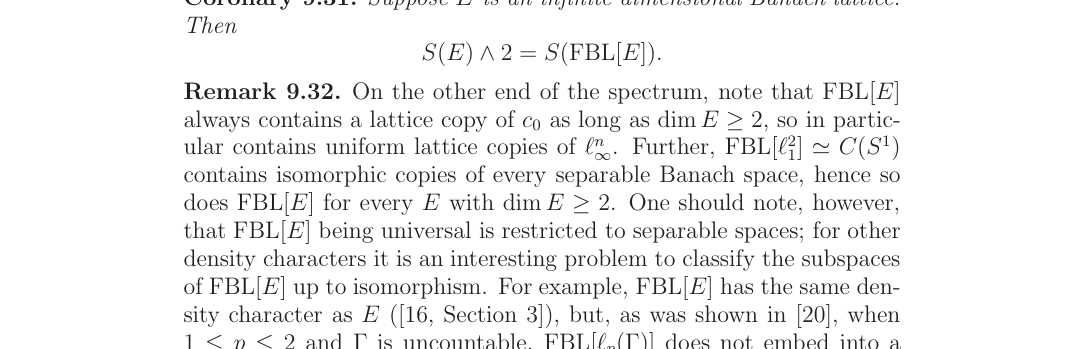
\includegraphics[width=0.92\linewidth]{figures/supporting_remark_crop.png}
\end{center}

Since \(\ellone\) is separable, \(\FBL[E]\) contains a subspace isomorphic
to \(\ellone\) whenever \(\dim E\ge 2\). If \(\dim E=0\) then \(\FBL[E]\)
is trivial, and if \(\dim E=1\) the free vector lattice generated by one
vector has only the positive and negative parts of one generator, so its
Banach-lattice completion is finite-dimensional. Thus the only
infinite-dimensional free Banach lattice cases are covered by \(\dim E\ge2\).

\emph{\(C(K)\)-spaces with a nontrivial component.}
Let \(K_0\) be a connected component of \(K\) containing two distinct points
\(s,t\). Since compact Hausdorff spaces are normal, Urysohn's lemma gives
a continuous function \(f:K\to[0,1]\) with \(f(s)=0\) and \(f(t)=1\). The
image \(f(K_0)\) is a connected compact subset of \([0,1]\) containing
both \(0\) and \(1\), hence \(f(K_0)=[0,1]\). Therefore \(f:K\to[0,1]\)
is onto. The pullback map
\[
J:C[0,1]\longrightarrow C(K),\qquad J(g)=g\circ f,
\]
is a linear isometry. By the Banach--Mazur theorem, \(C[0,1]\) contains an
isomorphic copy of every separable Banach space, in particular \(\ellone\).
Thus \(C(K)\) contains an isomorphic copy of \(\ellone\).

\emph{Compact Hausdorff ANR case.}
De Pagter and Wickstead prove that if \(K\) is an absolute neighbourhood
retract in the category of compact Hausdorff spaces, then \(K\) has only
finitely many connected components \cite[Section 11]{dPW}. If such a \(K\)
is infinite and every component were a singleton, then \(K\) would be a finite
union of singletons, hence finite, a contradiction. Thus an infinite compact
Hausdorff ANR has a non-singleton component. The preceding paragraph applies.

Finally, the source paper proves that \(C(K)\) is \(1^+\)-projective exactly
when \(K\) is a compact Hausdorff ANR \cite[Theorem 1.4]{AMRA}. Therefore the
full projective \(C(K)\)-family appearing in the source paper satisfies the
conclusion of Problem 2 whenever it is infinite-dimensional.
\end{proof}

\section*{Verification Notes}

The first part is a literature-implied subcase: the supporting authors do not
state that they are answering Problem 2 of \cite{AMRA}, but their Remark 9.32
implies it for the entire \(\FBL[E]\) family after observing that \(\ellone\)
is separable and that the \(\dim E\le1\) cases are finite-dimensional.

The second part is a standard \(C(K)\) argument plus a topological theorem of
de Pagter--Wickstead. The standard argument proves that any compact Hausdorff
\(K\) with a non-degenerate connected component gives
\(C[0,1]\hookrightarrow C(K)\). The cited finite-components theorem then
ensures that every infinite compact Hausdorff ANR has such a component.

\section*{Limitations And Novelty Check}

This packet does not solve Problem 2 in full. The remaining open territory is
an arbitrary infinite-dimensional \(\infty\)-projective Banach lattice that
is neither visibly a free Banach lattice nor a projective \(C(K)\)-space.

On June 20, 2026, web searches for the exact Problem 2 wording and close
phrases such as \emph{projective Banach lattice contains ell\_1} and
\emph{infty-projective Banach lattice ell\_1} located the source paper and
related strong-Nakano, semiprojective, and free-lattice literature, but no
explicit full answer to Problem 2. The free-lattice part is therefore recorded
as an identified literature implication, not as a new proof of Remark 9.32.

\section*{Human Review Recommendation}

This packet should be reviewed as a likely valid partial answer. The main
points to check are the exact scope of Remark 9.32 in \cite{OTTT}, the
finite-dimensional exception for \(\dim E\le1\), and the use of
de Pagter--Wickstead's finite-components theorem for compact Hausdorff ANRs.

\begin{thebibliography}{9}

\bibitem{AMRA}
A. Avil\'es, G. Mart\'inez-Cervantes, and J. D. Rodr\'iguez Abell\'an,
\emph{On projective Banach lattices of the form \(C(K)\) and \(\FBL[E]\)},
J. Math. Anal. Appl. 489 (2020), no. 1, 124129; arXiv:2002.12423.

\bibitem{OTTT}
T. Oikhberg, M. A. Taylor, P. Tradacete, and V. G. Troitsky,
\emph{Free Banach lattices}, arXiv:2210.00614.

\bibitem{dPW}
B. de Pagter and A. W. Wickstead,
\emph{Free and projective Banach lattices},
Proc. Roy. Soc. Edinburgh Sect. A \textbf{145} (2015), no. 1, 105--143;
arXiv:1204.4282.

\end{thebibliography}

\end{document}
